\FloatBarrier
\begin{figure}[H]
\begin{minipage}[b]{0.5\textwidth}
\centering
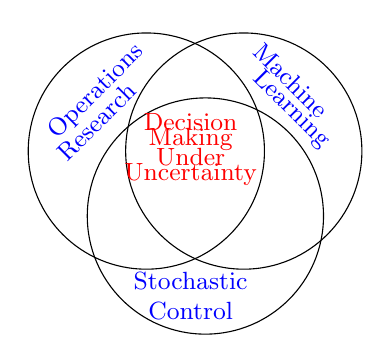
\begin{tikzpicture}[scale=0.75,font=\small,axis/.style={very thick, ->}]
\draw [] (0.9,0.5) circle (2);
\draw [] (-0.75,0.5) circle (2);
\draw [] (.25,-0.6) circle (2);
%\draw [] (-0.5,0.5) circle (2);
%\draw [] (0.5,-0.5) circle (2);
%\draw [] (-0.5,-0.5) circle (2);

\node[red] at(0,1){Decision};
\node[red] at(0,0.7){Making};

\node[red] at(0,0.4){Under};
\node[red] at(0,0.1){Uncertainty};

\node[blue,rotate=-45] at(1.7,1.7){Machine};
\node[blue,rotate=-45] at(1.7,1.2){Learning};

\node[blue,rotate=45] at(-1.6,1.5){Operations};
\node[blue,rotate=45] at(-1.6,1.0){Research};

\node[blue] at(-0,-1.7){Stochastic};
\node[blue] at(-0,-2.2){Control};
\end{tikzpicture}
\label{plan}
\captionsetup{font=footnotesize}
\captionof{figure}{Decision making under uncertainty is at the heart of many important areas such as Machine Learning, Operations Research and Stochastic Control.}
\end{minipage}
\begin{minipage}[b]{0.5\textwidth}

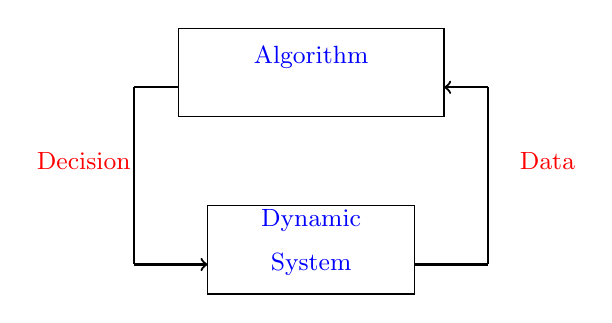
\begin{tikzpicture}[scale=0.75,font=\small,axis/.style={very thick, ->}]
\draw [black](-2.25,-1.25) rectangle (2.25,0.25);
\node[blue] at(0,-0.25) {Algorithm};
%\node[black] at(0,-0.75) {};

\draw [black](-1.75,-4.25) rectangle (1.75,-2.75);
\node[blue] at(0,-3) {Dynamic};
\node[blue] at(0,-3.75) {System};

\node[red] at(4,-2){{Data}};

\node[red] at(-3.85,-2){Decision};

\draw[thick,-](-2.25,-0.75)--(-3,-0.75);
\draw[thick,-](-3,-0.75)--(-3,-3.75);
\draw[thick,->](-3,-3.75)--(-1.75,-3.75);

\draw[thick,->](3,-0.75)--(2.25,-0.75);
\draw[thick,-](3,-3.75)--(3,-0.75);
\draw[thick,-](1.75,-3.75)--(3,-3.75);
\end{tikzpicture}
\captionsetup{font=footnotesize}
\captionof{figure}{The paradigm of data-driven approach to decision making is characterized by `system-in-loop' or `feedback' control. }
\end{minipage}
\end{figure}
